\chapter{Sistemas SCADA}
\label{chap:scada}

    Sistemas de Supervisão e Aquisição de Dados, do inglês, \gls{SCADA}, consistem basicamente de \textit{softwares} que monitoram e operam partes de um ou mais processos, através de unidades de aquisição de dados, como o \gls{CLP}, que por sua vez, conectado fisicamente ao servidor \gls{SCADA} e aos atuadores, utiliza protocolos de comunicação como os citados na seção \ref{sec:automacao-industrial} para obtenção e armazenamento destas informações. Com o domínio sobre as informações do processo, esta ferramenta é capaz de apresentar através de uma \gls{IHM} e de forma simplificada, valores e estados gerais do processo que se deseja atuar, desta forma, obtêm-se um maior controle sobre a tarefa, pois é possível centralizar a leitura de todos os sensores atuantes, a categorização e histórico destes dados, além da priorização de pendências do processo neste único sistema, reduzindo assim a necessidade um maior número de trabalhadores especializados que desempenhem a mesma função. \cite{WhatScada}
    
    O \gls{SCADA} apresenta uma série de vantagens, dentre elas: (i) redução de custos, devido a possibilidade de geração de relatórios detalhados úteis ao planejamento estratégico, evidenciando possíveis vícios do processo produtivo, (ii) maior desempenho na produção, por determinar os valores ótimos de trabalho, (iii) confiabilidade e continuidade, devido a existência de alarmes críticos, ou seja, notificações visuais ao operador, quando alguma variável ou condição do processo esteja em desacordo com o padrão de operação, desta forma, possíveis problemas que ocasionariam uma maior parada na produção, são mitigados com intervenções de forma quase imediata pelo operador caso sejam necessárias, trazendo assim vantagem competitiva.
    
    Todas as informações do processo podem ser coletadas e armazenadas em tempo real em um banco de dados, podendo serem implementadas no sistema de gestão empresarial da empresa ou utilizadas para cálculos mais complexos, sendo o último realizado por outras máquinas para garantir a que o \gls{SCADA} não tenha seu desempenho prejudicado.
    Uma representação básica do sistema \gls{SCADA} é ilustrada na Figura \ref{fig:figura-scada1}, ao qual todas as informações do processo são centralizadas e exibidas de forma simplificada ao colaborador. 
    
    \begin{figure}[!h]
	\Caption{\label{fig:figura-scada1} Arquitetura física básica do SCADA.}
	%\centering
	\UFCfig{}{
		\fbox{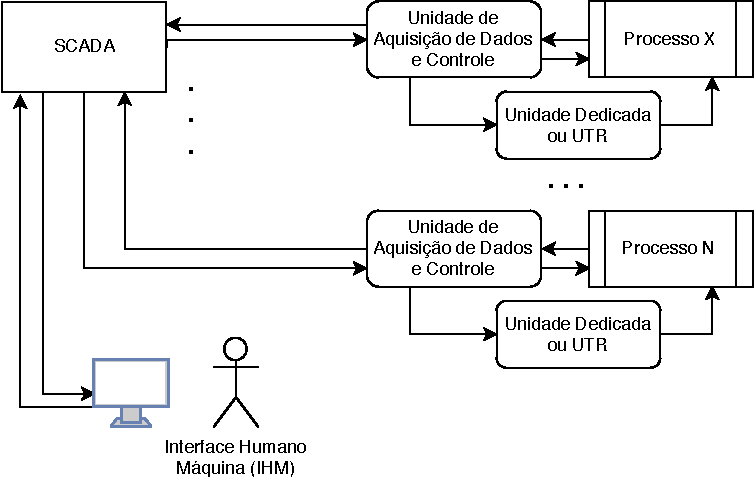
\includegraphics[width=14cm]{figuras/figura-scada1.pdf}}
	}{
		\Fonte{O autor}
	}	
    \end{figure}
    
\section{SCADA WEB}
\label{sec:scadaweb}

Rede Mundial de Computadores (\gls{WEB}), é como se designa o sistema de hiperligações e marcação de texto que permitem a disponibilidade de conteúdo através da \textit{internet}, como: páginas de texto, documentos, músicas, entre outros \cite{W3C}. O \gls{SCADA} \gls{WEB} é uma versão elaborada do SCADA convencional, onde os dados são transferidos para servidores na \textit{internet} e posteriormente processados, integrados às demais plataformas e/ou vistos em páginas WEB. A transição do SCADA para \gls{SCADA} \gls{WEB} ocorre principalmente devido à superação de uma baixa largura de banda e restrições de comunicação como ocorria antigamente. Os avanços tecnológicos possibilitaram a rápida expansão dos canais de dados através da \textit{internet}, onde até mesmo a transmissão de informações em tempo real, não é mais um fator limitante. \cite{ScadaWebSimp}

Sistemas \gls{SCADA} com base na \textit{internet} podem se tornar uma parte importante do funcionamento de sistemas de controle, onde o \gls{XML} e outras formatos disponíveis, podem oferecer possibilidade de resolução de problemas de incompatibilidade que existiam no \gls{SCADA} convencional, onde as fontes de comunicação com o processo são físicas e tornam necessários protocolos de comunicação específicos ou adaptações como o \gls{OPC}. Esta transição também ocorre com os dispositivos utilizados, como \glspl{CLP} e outros, que passam à contar com comunicação \gls{TCP/IP} integrada, alguns deles já com possibilidade de conexão \textit{Wi-Fi}, permitindo a utilização de protocolos como o \gls{HTTP} e \gls{MQTT}, nativos da \gls{WEB}, diretamente do dispositivo, removendo grande parte da camada física. A Figura \ref{fig:figura-clp-wago} traz um exemplo da fabricante WAGO, com uma família de dispositivos que possuem conexão direta à internet, além de recursos de criptografia.

\begin{figure}[!h]
\Caption{\label{fig:figura-clp-wago} Família de Dispositivos com Comunicação Integrada da fabricante WAGO.}
%\centering
\UFCfig{}{
	\fbox{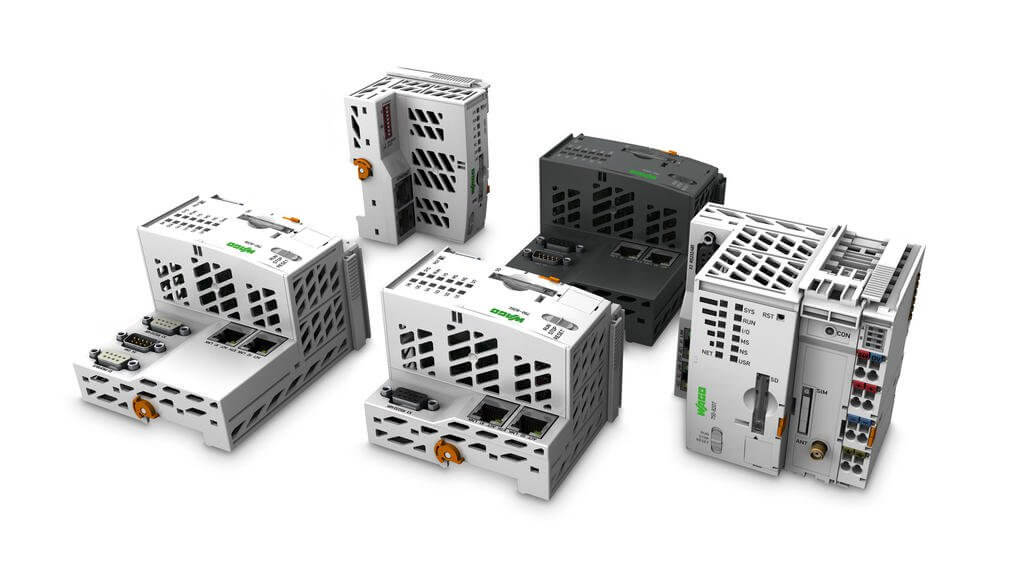
\includegraphics[width=10cm]{figuras/clp-wago.jpg}}
}{
	\Fonte{\cite{WAGO}}
}	
\end{figure}

Independente de como são obtidas as informações, a visualização se dá de forma mais familiar ao usuário, onde antes seria feita através de uma \gls{IHM} física, este ato se reduz à um simples \textit{smartphone} ou página no navegador simulando esta interface, sem ser necessária a instalação de qualquer \textit{software} adicional. A convergência das novas tecnologias, afeta drasticamente a supervisão destas informações, possibilitando controle distribuído e a possibilidade de armazenamento destas informações em qualquer lugar do mundo, com uma ampla capacidade de recursos \cite{ScadaWebInterOp}.

A implementação de um \gls{SCADA} \gls{WEB}, não só abre possibilidade de armazenamento de dados em várias localizações, como também eleva a capacidade de recursos computacionais à um nível muito superior, devido à possibilidade de utilização de servidores em nuvem - interligação de vários servidores através da internet formando um núcleo único de processamento - é possível controlar além de grupos de processos, grupos de plantas em único sistema. Segundo \cite{ScadaNextGer}, a nova geração do \gls{SCADA} pode modificar significamente a forma de projetar e implementar os processos industriais no futuro, onde o sistema terá que lidar com uma quantidade muito superior de dados distribuídos e informações em tempo real para tomar as decisões baseadas neste dados com informações internas e externas. A \gls{IHM} fica não mais limitada à um local físico, mas acessível através de todos os computadores, \textit{smartphones} e \textit{tablets} conectados à \textit{internet}, permitindo a colaboração simultânea na supervisão do processo. Com o uso de várias plantas simultâneamente, há a possibilidade de implementação de uma rotina por prioridades, dependendo das necessidades dinâmicas de cada cliente.  Poucas são as desvantagens de um sistema \gls{SCADA} \gls{WEB}, uma delas, é a perda de robustez do sistema devido as informações e controle serem feitos à distância através da rede, tendo que serem considerados atraso em transporte que, apesar de ser irrisório para a maioria das aplicações, podem chegar a ser um problema para outras. Uma representação básica do sistema \gls{SCADA} \gls{WEB} é ilustrada na Figura \ref{fig:figura-scada-web1}, onde as informações de um grupo de plantas são centralizadas e exibidas de forma simplificada ao colaborador.

    \begin{figure}[!h]
\Caption{\label{fig:figura-scada-web1} Arquitetura de um SCADA WEB.}
%\centering
\UFCfig{}{
	\fbox{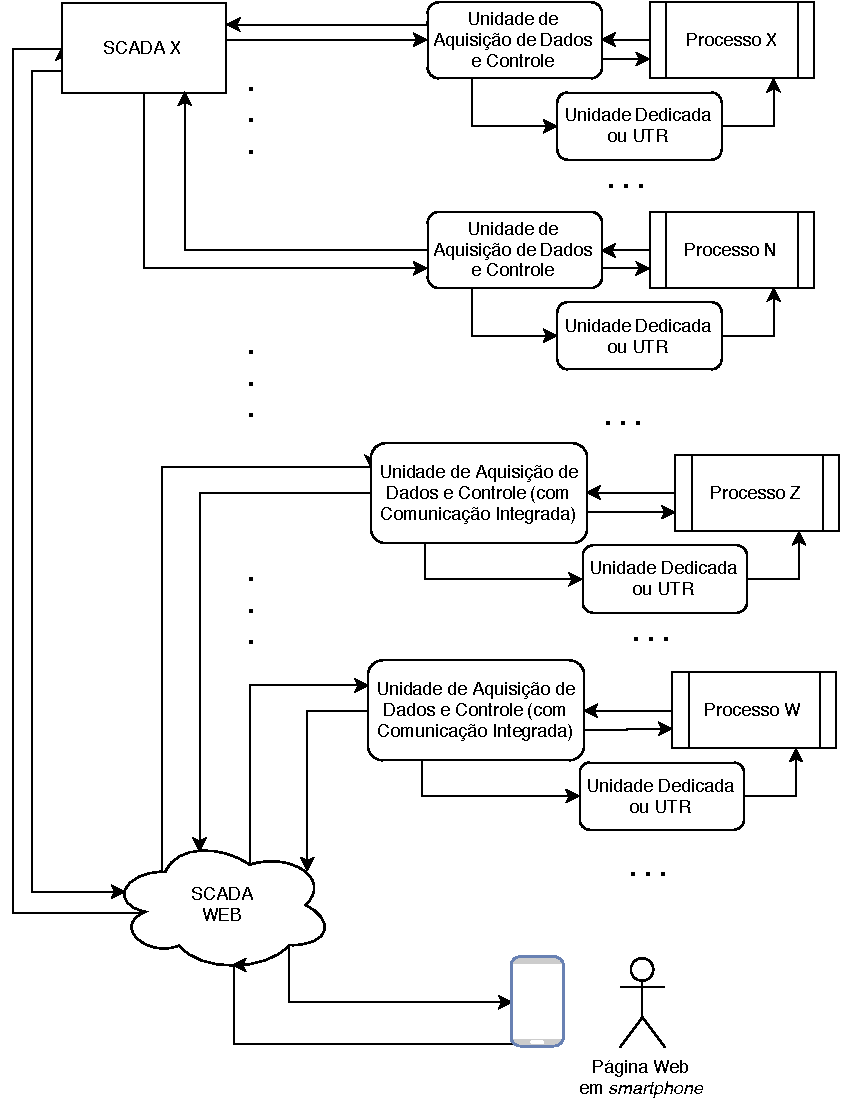
\includegraphics[width=14cm]{figuras/figura-scada-web1.pdf}}
}{
	\Fonte{O autor}
}	
\end{figure}

\section{Sistemas SCADA disponíveis no mercado}
\label{sec:sistemas-scada}

\subsection{Sistemas proprietários}
\label{sec:sistemas-scada-proprietarios}

\subsubsection{Elipse E3}
\label{sec:elipse}

    O Elipse E3 \cite{Elipse}, desenvolvido pela empresa Elipse Software, representa a terceira geração do \gls{SCADA}. Utiliza o conceito de múltiplas camadas, onde incluem: servidores, regras de aplicação ou de negócio e estações clientes. O sistema é composto por 3 aplicações: 
    
    \begin{alineascomponto}
    	\item \textit{E3Server}: é o servidor das aplicações, em que se gerencia todos os processos de execução do \textit{software} e processa a comunicação entre eles. Suas ações são basicamente: envio das informações gráficas e dados para o cliente, gerenciamentos dos processos de E/S e comunicação com os diversos pontos de aquisição, controle da cópia de produtos, cliente e servidor OPC e sincronismo de alarmes e bases de dados. Permite, também, a distribuição deste serviço entre várias máquinas de acordo com a necessidade, com objetivo de manter a continuidade em uma eventual falha.
    	\item \textit{E3Viewer}: responsável pela interface de operação e visualização da aplicação que se encontra no E3Server, com operação local ou via \textit{intranet}/\textit{internet}, pode ser acessado por diversas plataformas como: Mac OS, Linux, Windows CE ou ainda, há a possibilidade de utilização do E3WebServer para gerenciamento adicional do acesso via Internet.
    	\item \textit{E3Studio}: ferramenta para configuração do sistema, servindo como plataforma universal do desenvolvimento. A configuração e execução compartilham da mesma base de dados, de forma que as edições das aplicações podem ser enviadas em \textit{runtime}, sem ser necessário a parada da aplicação, independente de ser feita local ou remotamente. É possível a edição de mais de um aplicativo ao mesmo tempo ou a edição ser feita por mais de uma pessoa devido compartilharem o mesmo servidor. Possui ferramentas, como: editores de telas, relatórios e \textit{scripts}.
    \end{alineascomponto}
    
    \begin{figure}[!h]
	\Caption{\label{fig:figura-elipse-e3} Demonstração da tela de processo do \textit{software} Elipse E3.}
	%\centering
	\UFCfig{}{
		\fbox{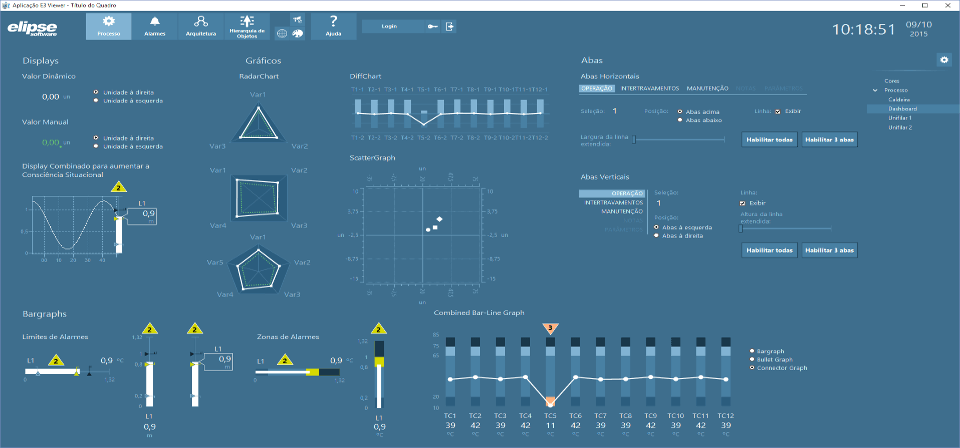
\includegraphics[width=15cm]{figuras/elipse-e3.png}}
	}{
		\Fonte{\cite{Elipse}.}
	}	
    \end{figure}

    
    Outras informações importantes:
    
    \begin{alineascomponto}
    	\item Possui drivers para comunicação com mais de 300 tipos de dispositivos e sistemas, sejam eles proprietários ou \gls{OPC}, além de produzir drivers sob encomenda.
    	\item Possui interfaces específicas para Access (.MDB), SQL Server/MSDE, Oracle ou acesso genérico através de padrões ADO e ODBC, faz acesso à base de dados corporativas fazendo o interfaceamento entre o processo e sistemas administrativos, de produção, manutenção e gestão.
    \end{alineascomponto}
    
\subsubsection{InduSoft Web Studio®}
\label{sec:indusoft}

    O InduSoft Web Studio® \cite{InduSoft}, desenvolvido pela empresa InduSoft, fornece componentes básicos de automação para o desenvolvimento de \glspl{IHM}, sistemas \glspl{SCADA} e soluções de instrumentação embarcada. O sistema é composto por 2 aplicações:
    
    \begin{alineascomponto}
        \item \textit{Server}: é o servidor das aplicações, em que se gerencia todos os processos de execução do \textit{software} e processa a comunicação entre eles. Suas ações são basicamente: envio das informações gráficas e dados para o cliente, gerenciamentos dos processos de entrada e saída,  comunicação com os diversos pontos de aquisição, controle da cópia de produtos, servidor OPC e sincronismo de alarmes e bases de dados.
    	\item \textit{IoTViewer}: responsável pela interface de operação e visualização da aplicação que se encontra no \textit{Server}, com operação local ou via \textit{intranet}/\textit{internet}.
    \end{alineascomponto}

    \begin{figure}[!h]
	\Caption{\label{fig:figura-indusoft} Demonstração da tela de processo do \textit{software} InduSoft Web Studio®.}
	%\centering
	\UFCfig{}{
		\fbox{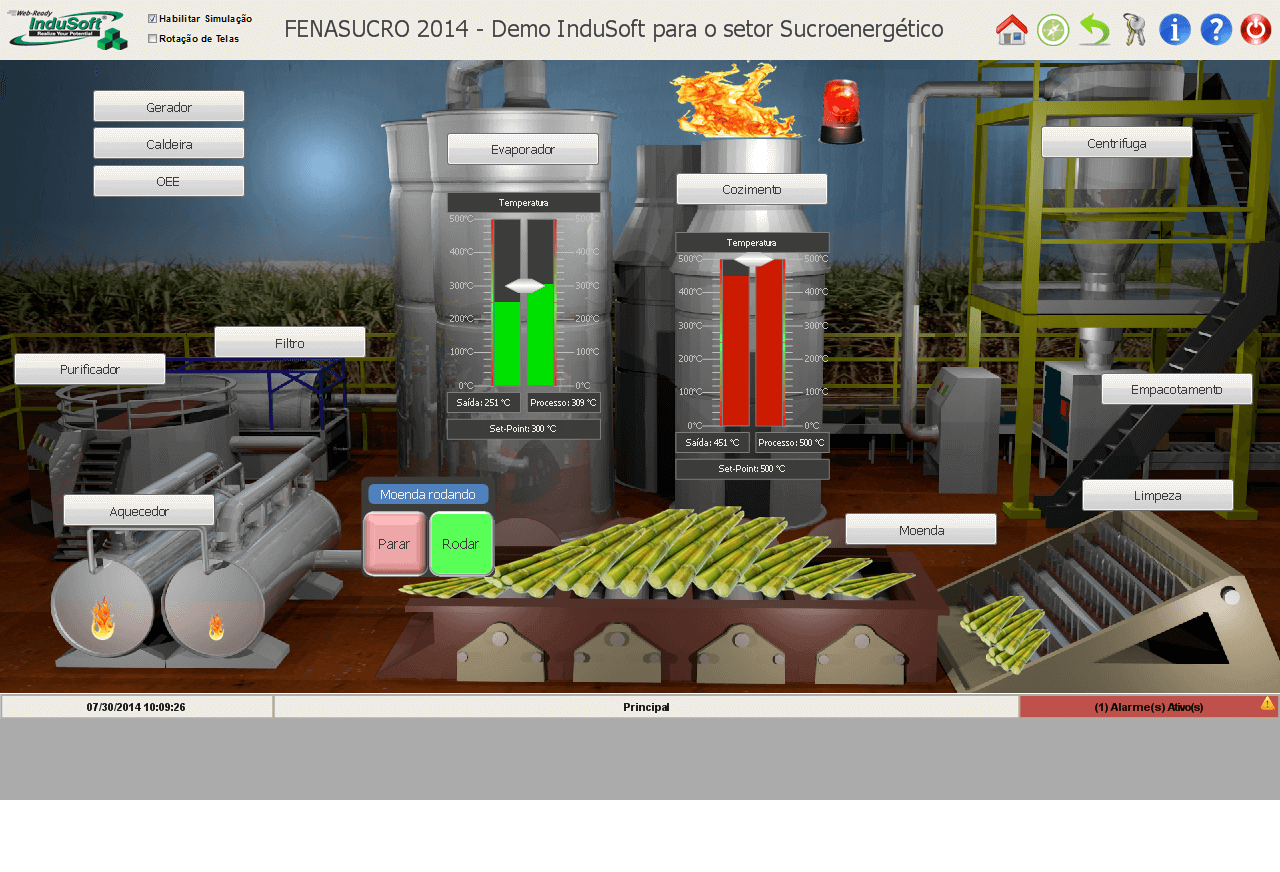
\includegraphics[width=15cm]{figuras/indusoft.png}}
	}{
		\Fonte{\cite{InduSoft}.}
	}	
    \end{figure}
    
    Outras informações importantes:
    
    \begin{alineascomponto}
    	\item A aplicação \textit{Server} suporta as plataformas \textit{Microsoft}, como: \textit{Windows CE, Mobile, XP Embedded e Server}, enquanto a aplicação cliente, o \textit{IoTView}, pode também suportar plataformas, como: \textit{Linux e VXWorks}.
    	\item Permite visualização de processo através de Navegador \gls{WEB}, podendo ser acessado através de celulares ou computadores de mesa, seja em rede local ou pela \textit{internet}.
    	\item Possui suporte para \gls{CLP} ou controlador e drivers para comunicação com mais de 200 tipos de dispositivos e sistemas, sejam eles proprietários ou \gls{OPC}, além de comunicação por \gls{TCP/IP}.
    	\item Alarmes podem ser enviados via \textit{e-mail}, celulares ou através do próprio navegador.
    	\item Permite acesso à base de dados corporativas fazendo o interfaceamento entre o processo e sistemas administrativos, de produção, manutenção e gestão.
    \end{alineascomponto}


\subsection{Sistemas de código aberto}
\label{sec:sistemas-aberto}

\subsubsection{ScadaBR}
\label{sec:scadabr}

    O ScadaBR \cite{ScadaBR} é um \textit{software} livre e de código-fonte aberto. Abrange profissionais de automação, universidades, escolas técnicas e empresas de todos os portes. O projeto foi iniciado em 2006, por iniciativa da empresa MCA Sistemas com sede em Florianópolis - SC, que com o auxílio de outras empresas, a fundação CERTI e a Universidade Federal de Santa Catarina - UFSC, desenvolveram o sistema de forma completa em português baseado no \textit{software} Mango. Possui apoio da FINEP, SEBRAE e CNPq, que também, financiaram a iniciativa durante 2 anos.

    \begin{figure}[!h]
	\Caption{\label{fig:figura-scadabr} Demonstração de telas, incluindo a de processo, do \textit{software} ScadaBR.}
	%\centering
	\UFCfig{}{
		\fbox{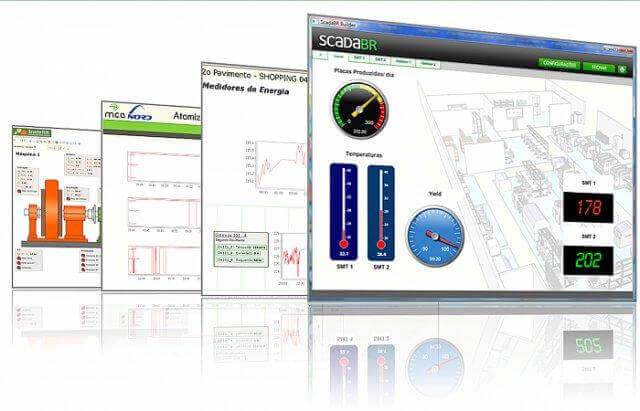
\includegraphics[width=12cm]{figuras/scadabr.jpg}}
	}{
		\Fonte{\cite{ScadaBR}.}
	}	
    \end{figure}
    
    Outras informações importantes:
    
    \begin{alineascomponto}
	    \item A aplicação \textit{Server} suporta diferentes plataformas, como: \textit{Windows} 32/64 bits e \textit{Linux}.
	    \item Permite visualização de processo através de Navegador \gls{WEB}, podendo ser acessado através de celulares ou computadores de mesa, seja em rede local ou pela \textit{internet}.
    	\item Possui mais de 20 protocolos de comunicação, como: Modbus \gls{TCP/IP} e Serial, \gls{HTTP}, etc.
    	\item Customização de \textit{scripts} para controle, automação, etc.
    	\item Possibilidade de cálculos com funções matemáticas, estatísticas etc, com as variáveis do processo.
    	\item Níveis de permissão de usuários, com controle de acesso.
    \end{alineascomponto}
    
\subsubsection{TANGO Controls}
\label{sec:tango}

    O TANGO Controls \cite{Tango} é um \textit{software} livre e de código-fonte aberto. Foi desenvolvido pelo \textit{European Synchrotron Radiation Facility} em Genebra, França e seu desenvolvimento já supera 20 anos de duração. Foi desenvolvido, principalmente, para necessidades de instalações de pesquisas, com o conceito agregado de ser criado um novo \textit{framework}. Pode ser executado de forma autônoma ou distribuída, local ou remota.

    \begin{figure}[!h]
	\Caption{\label{fig:figura-tango} Demonstração da tela de processo do \textit{software} TANGO Controls.}
	%\centering
	\UFCfig{}{
		\fbox{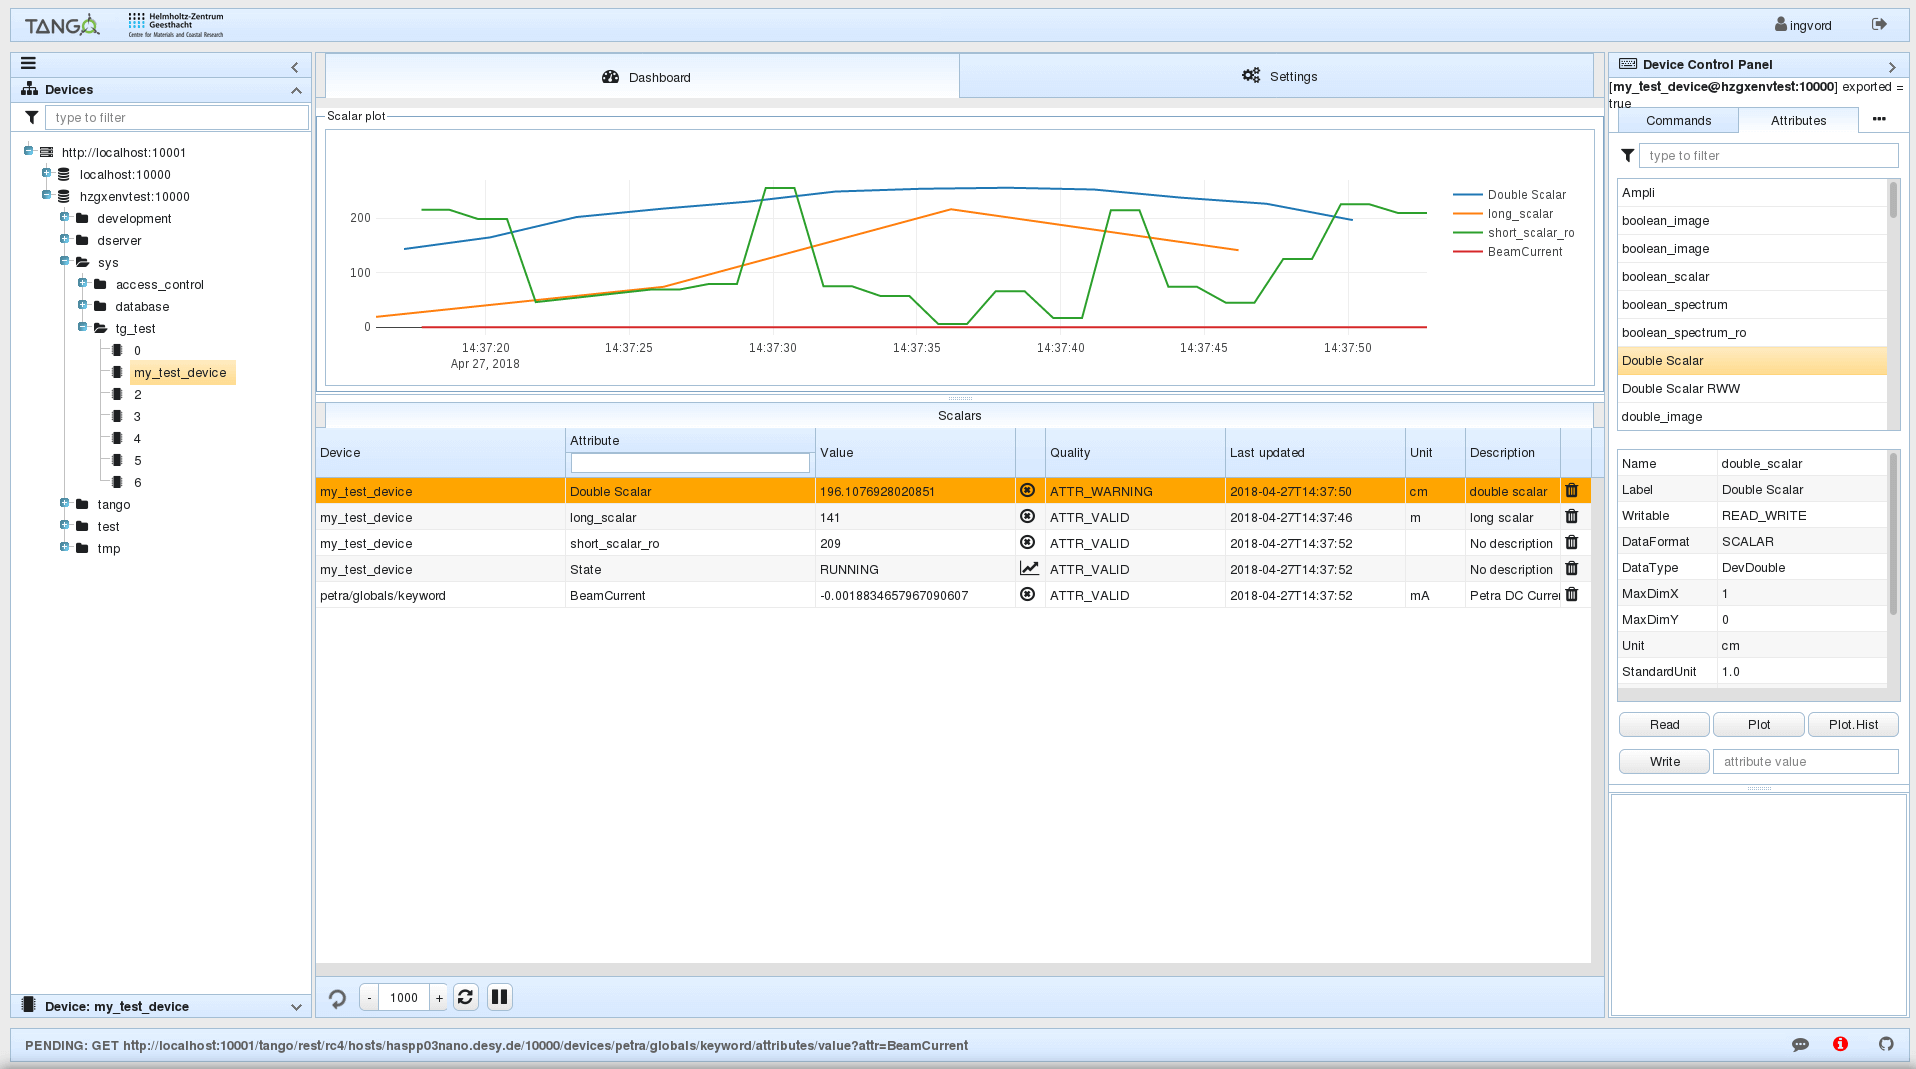
\includegraphics[width=15cm]{figuras/tango.png}}
	}{
		\Fonte{\cite{Tango}.}
	}	
    \end{figure}
    
    Outras informações importantes:
    
    \begin{alineascomponto}
	    \item Permite visualização de processo através de Navegador \gls{WEB}, podendo ser acessado através de celulares ou computadores de mesa, seja em rede local ou pela \textit{internet}.
    	\item Possui diversos \textit{drivers} de comunicação, disponibilizados de forma gratuita.
    	\item Permite a adição de funções analíticas para a tomada de decisões.
    	\item Encontra-se em fase de transição para atender a demanda \textit{IoT} industrial.
    \end{alineascomponto}
    
\subsubsection{Rapid SCADA}
\label{sec:rapidscada}

    O Rapid SCADA \cite{RapidSCADA} é um \textit{software} livre e de código-fonte aberto, desenvolvido pela empresa russa \textit{Rapid Software}.

    \begin{figure}[!h]
	\Caption{\label{fig:figura-rapidscada} Demonstração da tela de processo do \textit{software} Rapid SCADA.}
	%\centering
	\UFCfig{}{
		\fbox{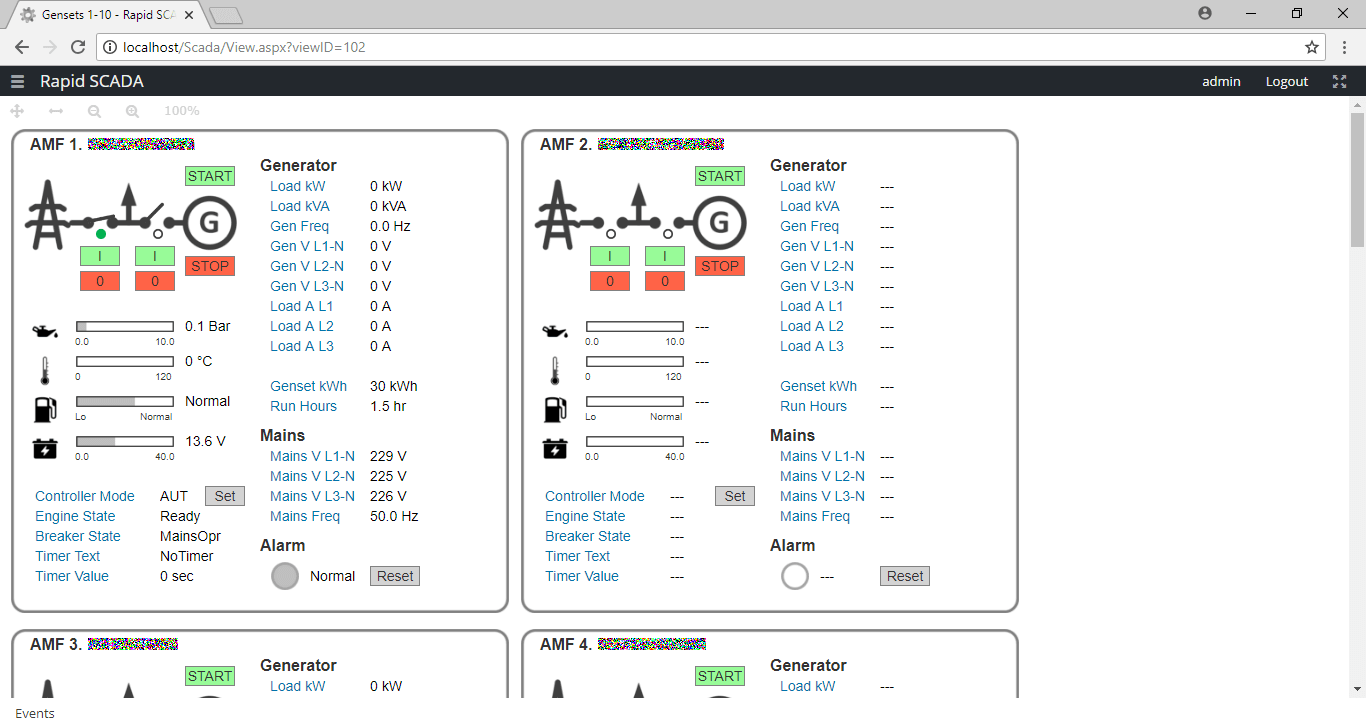
\includegraphics[width=15cm]{figuras/rapidscada.png}}
	}{
		\Fonte{\cite{RapidSCADA}.}
	}	
    \end{figure}
    
    Outras informações importantes:
    
    \begin{alineascomponto}
        \item É suportado por plataformas \textit{Windows} e \textit{Linux}.
	    \item O sistema possui uma interface de administração no modelo cliente/servidor e outra de monitoramento no formato \gls{WEB}.
	    \item Possui \textit{drivers} de comunicação, disponibilizados de forma gratuita, como: Modbus, \gls{OPC}, \gls{MQTT}, etc.
	    \item Níveis de permissão de usuários, com controle de acesso.
	    \item Alarmes de fogo e segurança, com avisos via interface.
	    \item A empresa cobra por serviços de treinamento e suporte na ferramenta, além de comercializar módulos de software adicionais.
    \end{alineascomponto}
    
\section{Síntese}
\label{sec:sintese-scada}

Apresentados os dispositivos e protocolos utilizados na indústria para a manutenção de processos industriais, neste Capítulo foram apresentados os tipos de sistemas \gls{SCADA} existentes assim como os principais \textit{softwares} disponíveis no mercado para esta funcionalidade. Com base em todo o desenvolvimento teórico apresentado, o capítulo seguinte traz a proposta de um sistema \gls{SCADA} baseado em nuvem com a capacidade de gerenciamento de múltiplos projetos na mesma estrutura.